
The telescope performance has been validated at CERN (120\,GeV pions) and DESY (1 to 6\,GeV positrons). 
In order to get realistic data description at DESY beam energies all scattering material between sensitive planes has to be taken into account. 
The precision of the track prediction at the DUT (plane \#3) based on five other telescope planes is shown in Figure\,\ref{fig:resolution}. 
The combination of the thickness of the telescope planes ($\unit{50}{\upmu\meter}$) with their hit position precision ($\sim\unit{3.5}{\upmu\meter}$)
 when minimising the distances to the Detector Under Test (DUT), 
 allows to sustain track pointing precision below $\unit{3}{\upmu\meter}$ for all electron (positron) energies above 2\,GeV and distance to the DUT shorter then 20\,mm (Figure\,\ref{fig:resolution}).

More stuff:


The figure of merit for a beam telescope is its resolution - both in time and in
space, as this defines the precision with which each track can be measured. The
timing resolution is largely dependent on the readout speed of the used
sensors, their buffer sizes and the data aquisition system. Spatial resolution
depends on the individual intrinsic sensor resolution, the number of planes in
each track and their position, as well as the multiple scattering of the beam
particles. The expression

\begin{equation}
\label{eq:telescoperesolutionequation}
\sigma_{\textrm{meas}}^2 = \sigma_{\textrm{DUT}}^2 + \sigma_{\textrm{Tel}}^2 +
\sigma_{\textrm{MS}}^2
\end{equation}

shows the contributing terms that have to be
considered~\cite{ref:eudetreport200902}. The measured residual width on a
DUT sensor plane is expressed by $\sigma_{\textrm{meas}}$,
$\sigma_{\textrm{DUT}}$ is the actual achievable resolution on the DUT plane,
$\sigma_{\textrm{Tel}}$ is the resolution of the telescope and
$\sigma_{\textrm{MS}}$ represents the contribution from multiple scattering.
In the following, all terms will be discussed.\\


The resolution of a telescope $\sigma_{\textrm{Tel}}$ can be expressed by

\begin{equation}
\sigma_{\textrm{Tel}}^2 = k \cdot \sigma_{\textrm{Intrinsic}}^2
\end{equation}

with the geometric scaling factor $k$ in turn written as

\begin{equation}
k = \frac{\sum_i^N z_i^2}{N \cdot \sum_i^N z_i^2 - \left( \sum_i^N z_i
\right)^2}
\end{equation}

assuming all $N$ telescope planes have the same intrinsic resolution
$\sigma_{\textrm{Intrinsic}}$~\cite{ref:eudetreport200902}. $z_i$ is then the
distance of the $i$-th telescope plane to the DUT positioned at $z=0$.\\

Multiple scattering is the term used to describe the deflection of a charged
particle traversing any medium. It depends on the particle energy and type
and the radiation length of the matter traversed~\cite{ref:scatteringhighland}.
The width of the angular scattering distribution can be expressed by

\begin{equation}
\label{eq:multiplescattering}
\Theta_{0} = \frac{13.6\,\mega\electronvolt}{\beta c p} \cdot z
\sqrt{x \per X_0}
\cdot \left( 1 + 0.038 \ln{\left( x \per X_0\right) } \right)
\end{equation}

according to~\cite{ref:PDG-2014}, with the particle velocity $\beta c$, momentum
$p$ and charge number $z$. The expression $x/X_0$ defines the thickness of the
scattering medium in radiation lengths, with values of $X_0 =
21.82\,\allowbreak\gram\per\centi\meter^2$ for silicon and $X_0 =
36.62\,\gram\per\centi\meter^2$ for dry air, according to~\cite{ref:x0values}.\\

Equation~\ref{eq:multiplescattering} shows, that the angular distortion due to
multiple scattering increases with the material budget and the inverse energy.
Therefore, at low-energy beams, such as the $6\,\giga\electronvolt$ DESY-II test
beam, it is advantageous to have very thin telescope sensors. As the beam
particles also interact with the atoms in the air, a contribution to the amount
of multiple scattering depending on the distance between sensor planes has to be
considered. At high-energy hadron beams ($> 100\,\giga\electronvolt$), which for
example are avaibale at the SPS facility at CERN, the contribution from multiple
scattering can be neglected.\\





Fullquote~\cite{ref:thomas}
\bigskip


\section{Telescope Performance}\label{sec:telescoperesolution}

To verify the performance of the {DATURA} telescope, measurements of the
achievable resolution were performed in $2012$, for different settings of beam
momentum, sensor threshold and sensor spacing. With the \texttt{datura-noDUT}
example included in the {EUTelescope} framework, which is described in detail in
section~\ref{sec:datura-nodut}, straight line tracks with hits in all six
telescope planes were sought. From these tracks, the unbiased residual
distribution of each sensor plane was calculated. To calculate this
distribution, each of the six telescope planes was iteratively considered as a
DUT. Within each iteration, tracks were calculated from the five non-DUT planes.
The unbiased residual distribution was then filled by the distance between the
hit position and the track extrapolation in the DUT plane. By using each
telescope plane as a DUT, equation~\ref{eq:telescoperesolutionequation} is
modified under the assumption that $\sigma_{\textrm{Intrinsic}} =
\sigma_{\textrm{DUT}} = \sigma_{\textrm{M26}}$, leading to

\begin{equation}
\label{eq:telescoperesolutionequation_2}
\sigma_{\textrm{meas}}^2 = \sigma_{\textrm{M26}}^2 \cdot \left( 1 + k \right) +
\sigma_{\textrm{MS}}^2\,.
\end{equation}


Figure~\ref{fig:residualexample1} shows an example of residual distributions for
a telescope sensor spacing of $20\,\milli\meter$, a beam momentum of
$5\,\giga\electronvolt$ and a sensor threshold setting of $6$. The residual
distributions for the outer planes $0$ and $5$ are wider than the distributions
obtained from the inner sensors. This is due to the fact that the track
extrapolation to the inner sensors is done from both sides, hence will be
comparatively more precise than for the outer sensors, where the extrapolation
can only be performed from one direction. In all cases, the distributions are
fitted with a Gaussian, from which the residual width $\sigma_{\textrm{meas}}$
is determined.\\

\begin{figure}[hbtp]
\centering
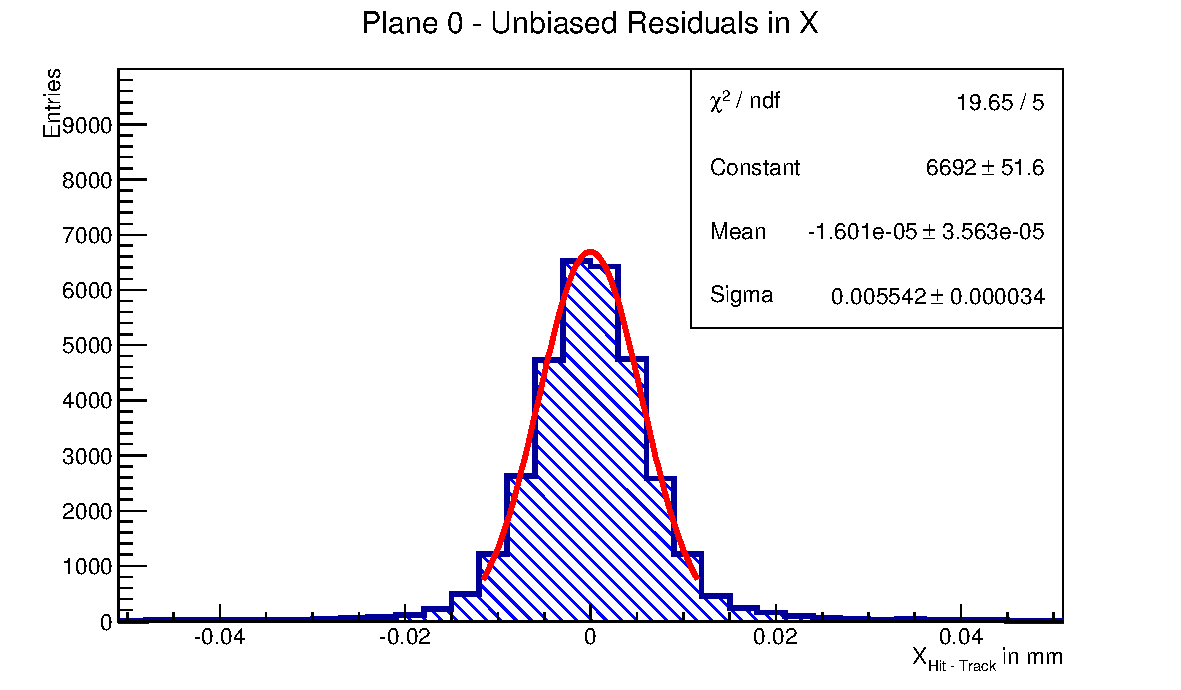
\includegraphics[width=0.45\textwidth]{gfk/chapter03/resis_upstream/0x.pdf}
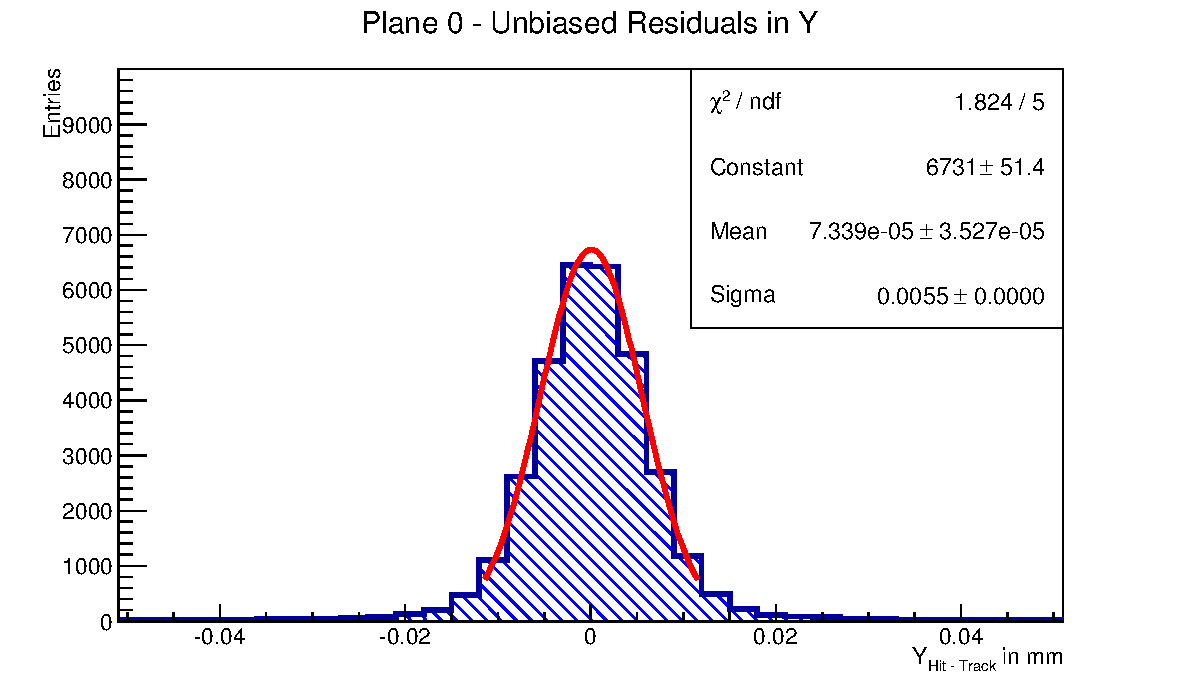
\includegraphics[width=0.45\textwidth]{gfk/chapter03/resis_upstream/0y.pdf}
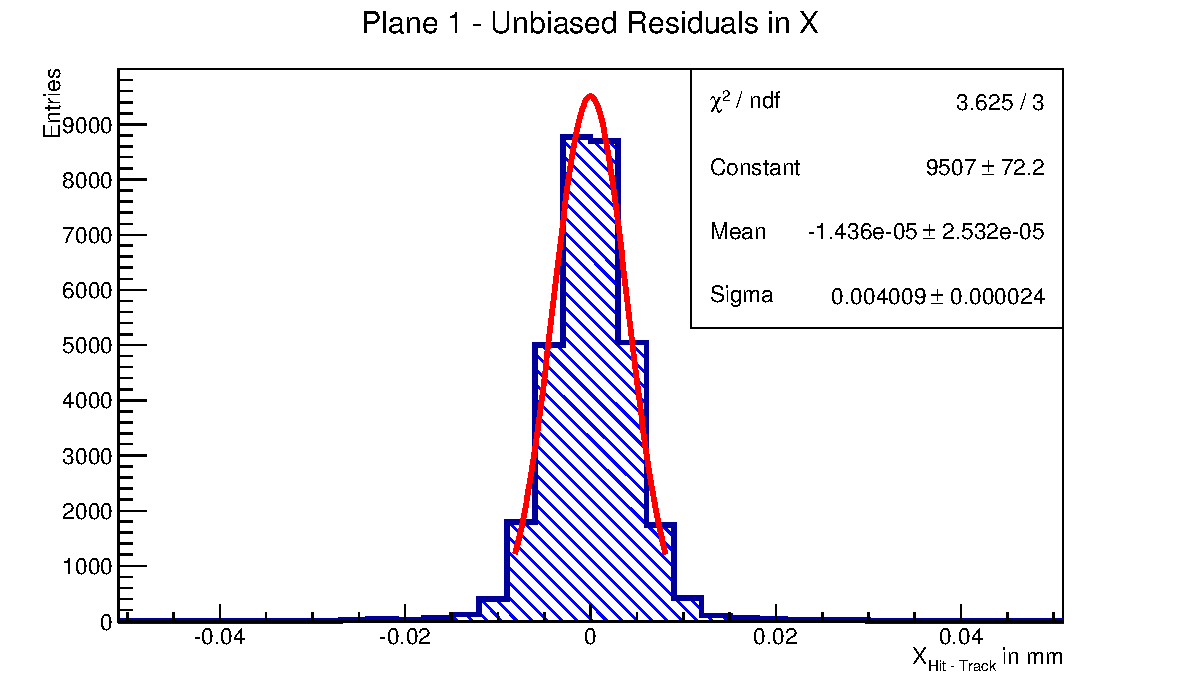
\includegraphics[width=0.45\textwidth]{gfk/chapter03/resis_upstream/1x.pdf}
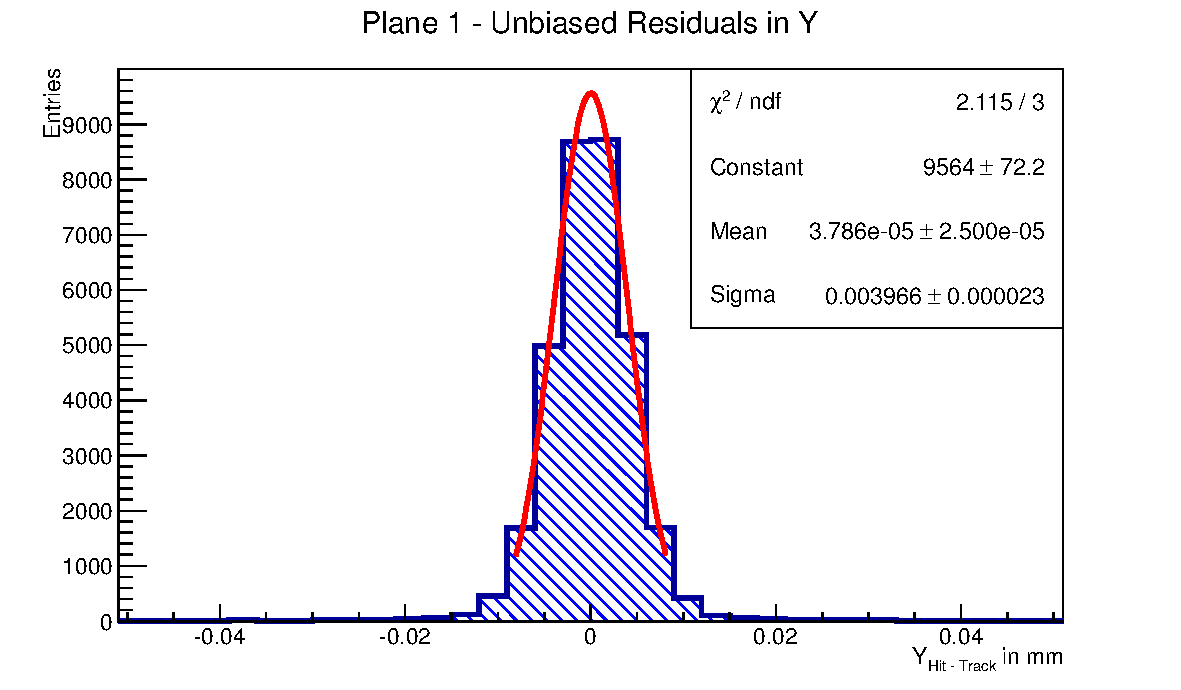
\includegraphics[width=0.45\textwidth]{gfk/chapter03/resis_upstream/1y.pdf}
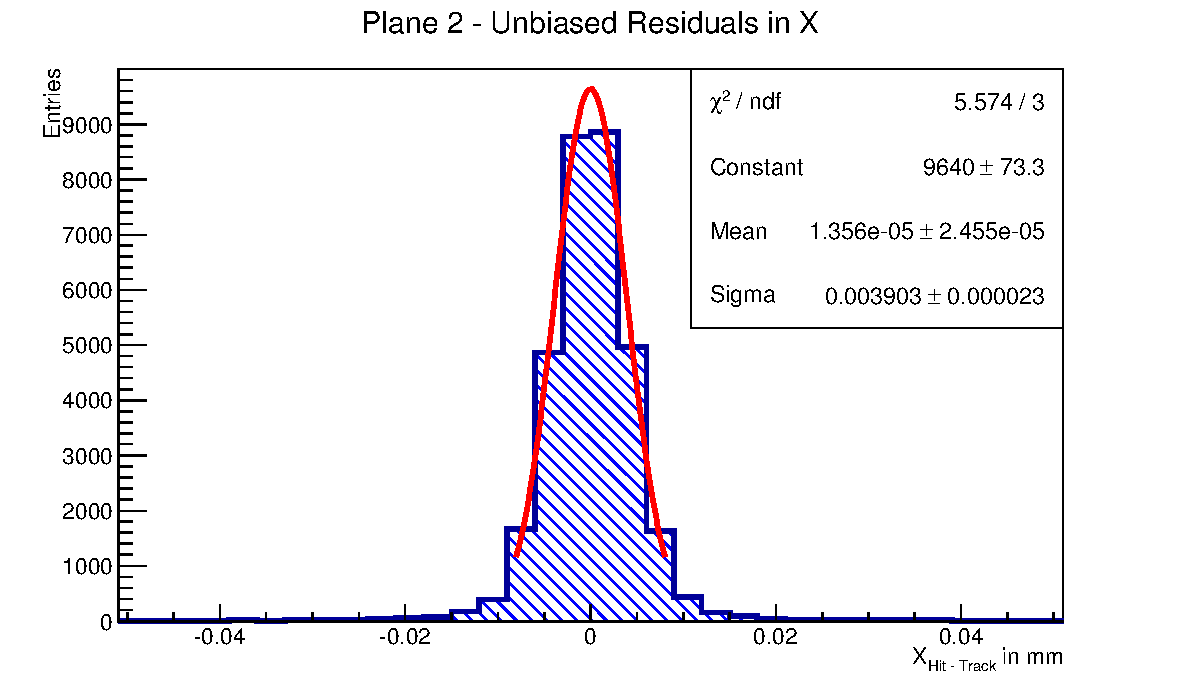
\includegraphics[width=0.45\textwidth]{gfk/chapter03/resis_upstream/2x.pdf}
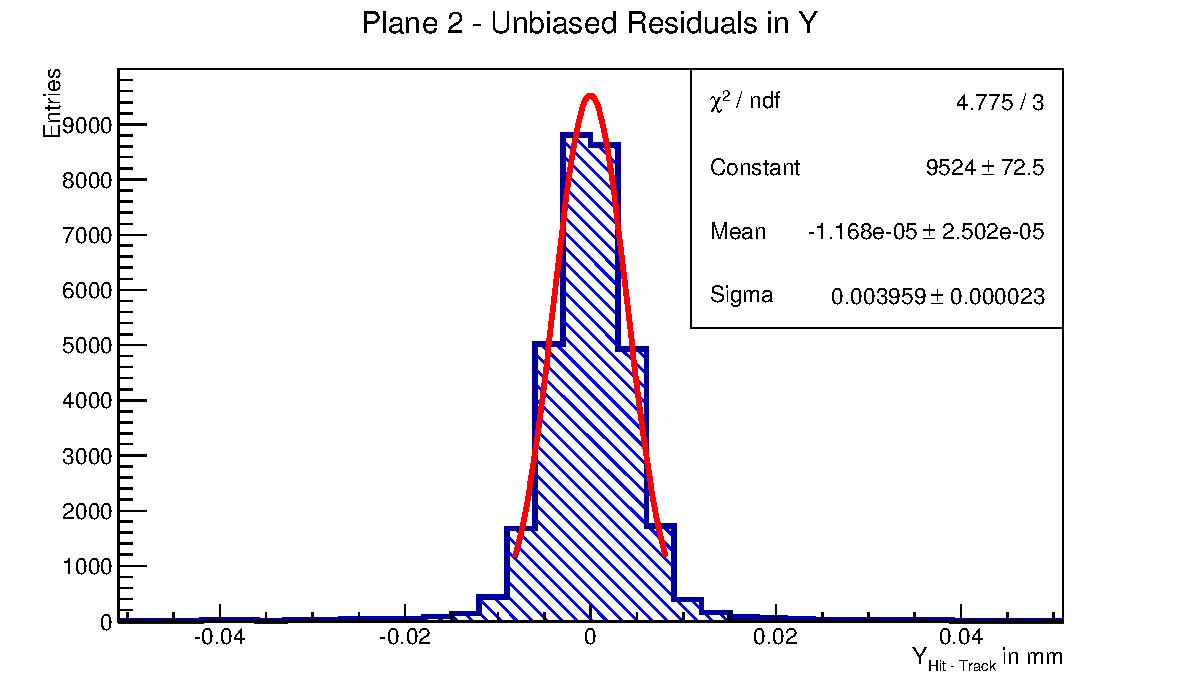
\includegraphics[width=0.45\textwidth]{gfk/chapter03/resis_upstream/2y.pdf}
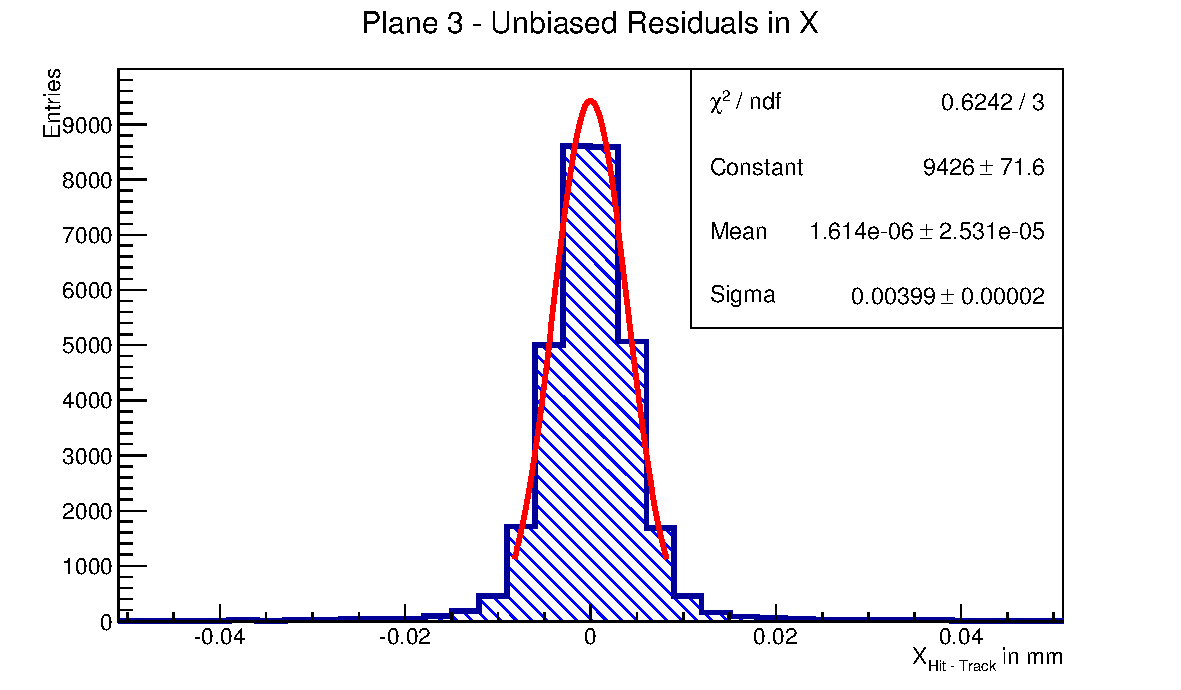
\includegraphics[width=0.45\textwidth]{gfk/chapter03/resis_downstream/3x.pdf}
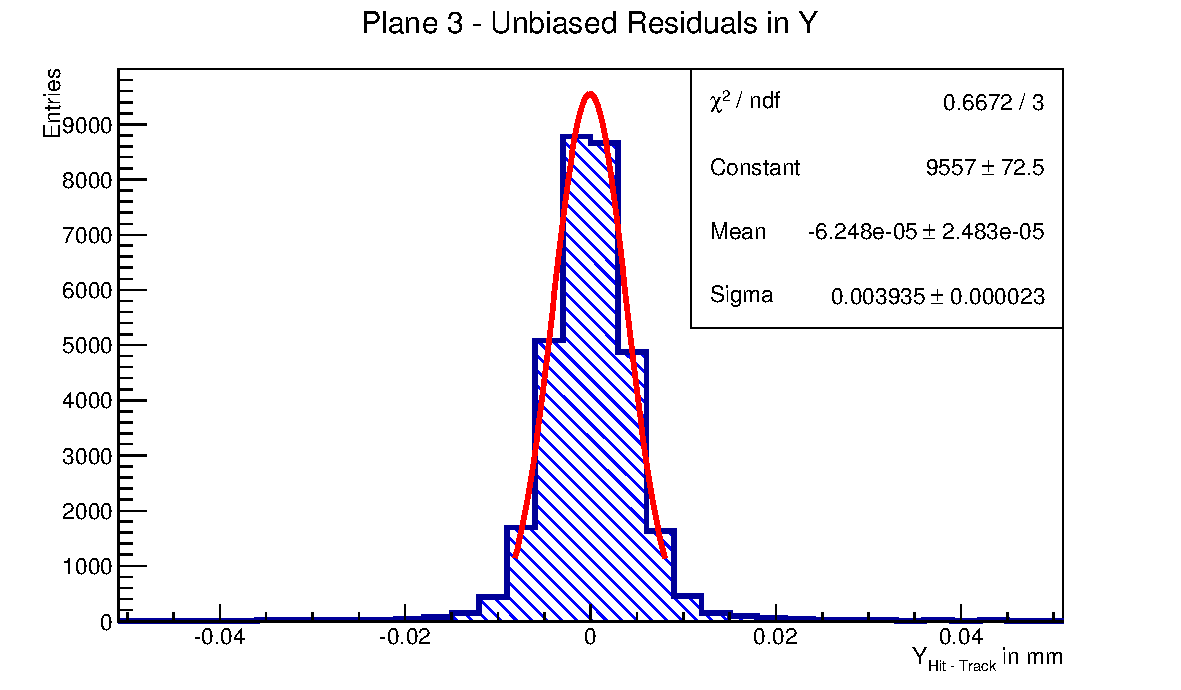
\includegraphics[width=0.45\textwidth]{gfk/chapter03/resis_downstream/3y.pdf}
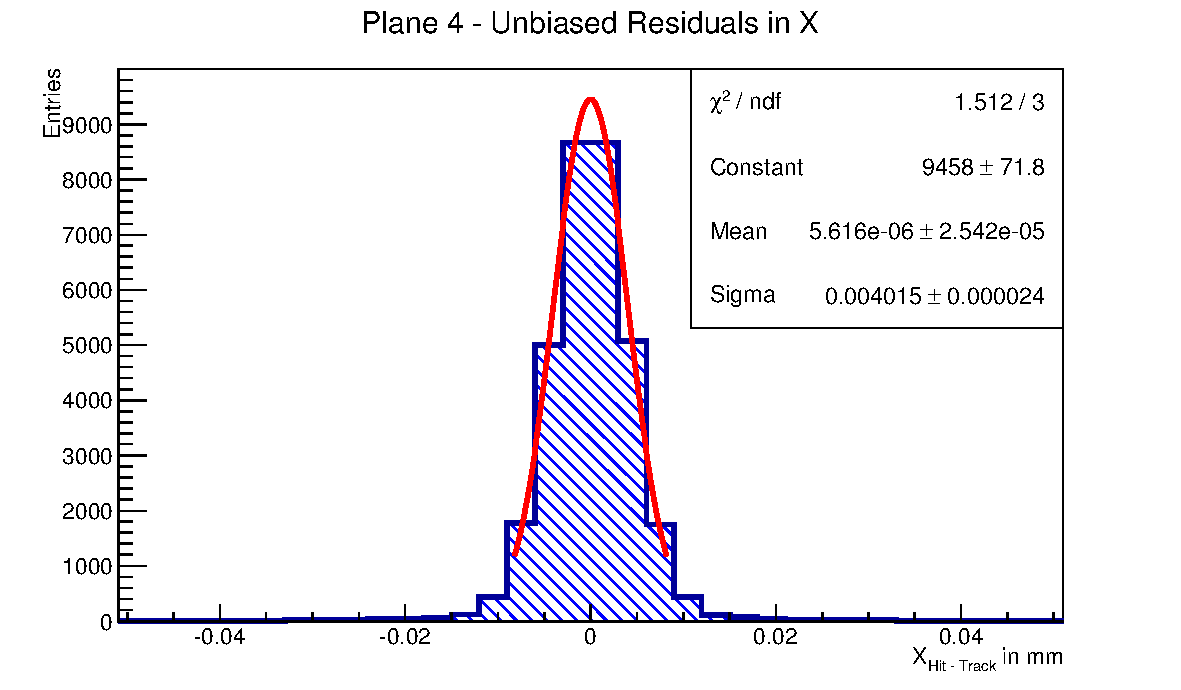
\includegraphics[width=0.45\textwidth]{gfk/chapter03/resis_downstream/4x.pdf}
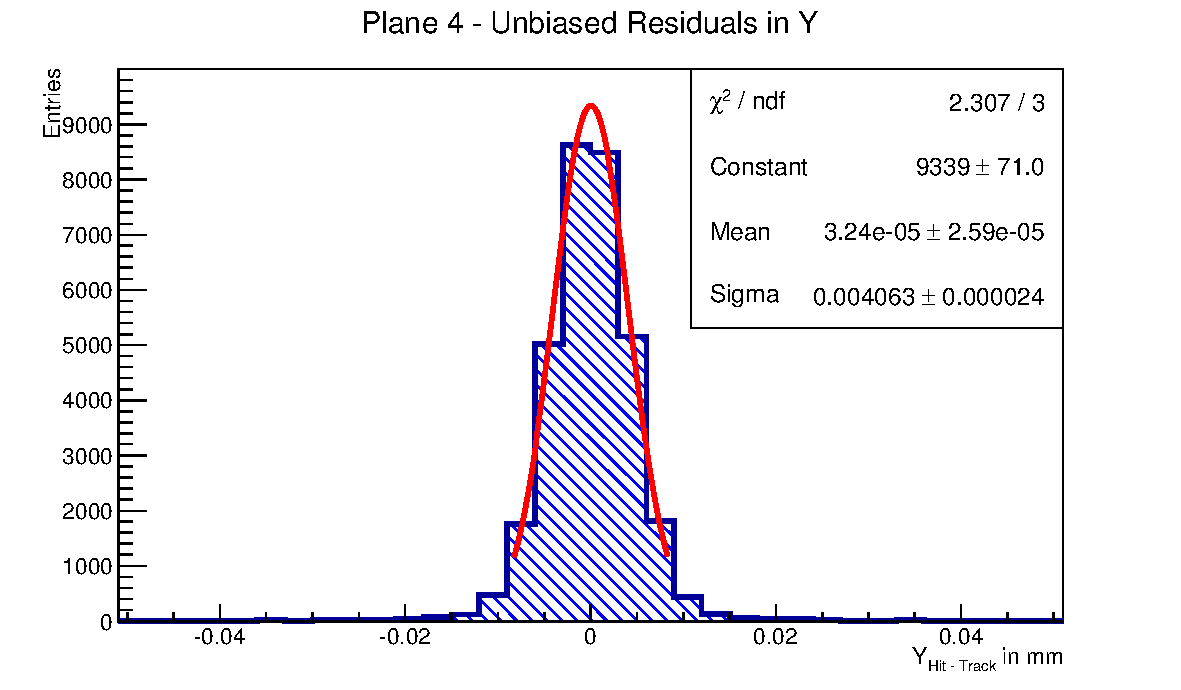
\includegraphics[width=0.45\textwidth]{gfk/chapter03/resis_downstream/4y.pdf}
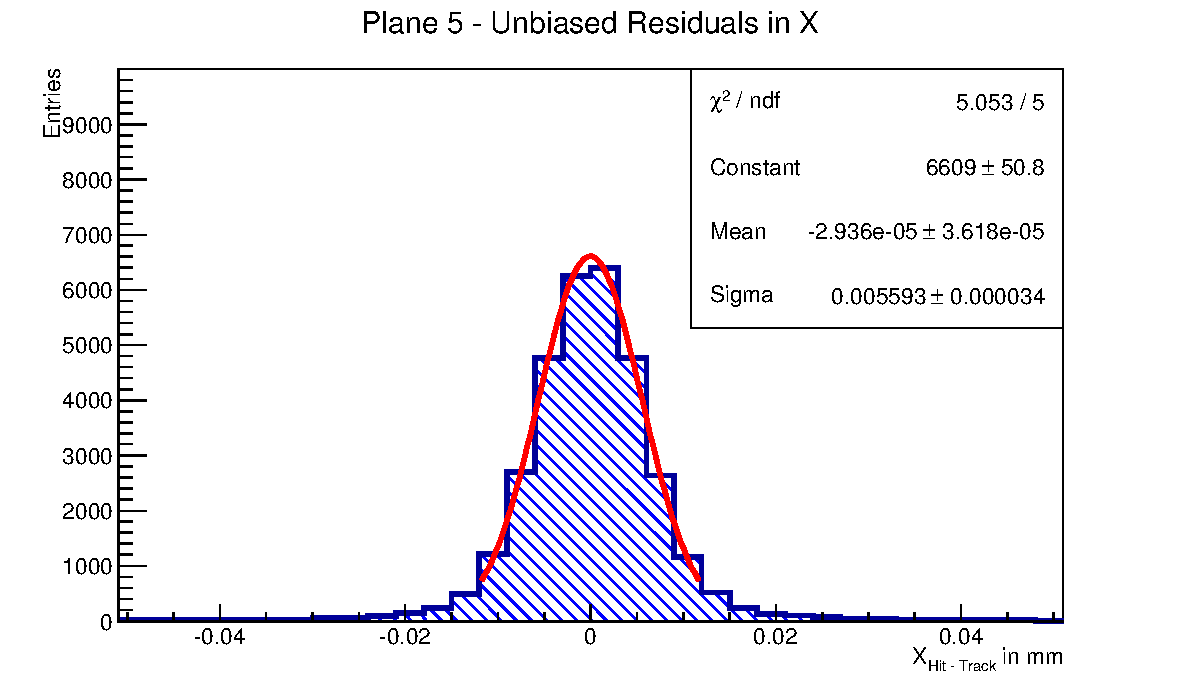
\includegraphics[width=0.45\textwidth]{gfk/chapter03/resis_downstream/5x.pdf}
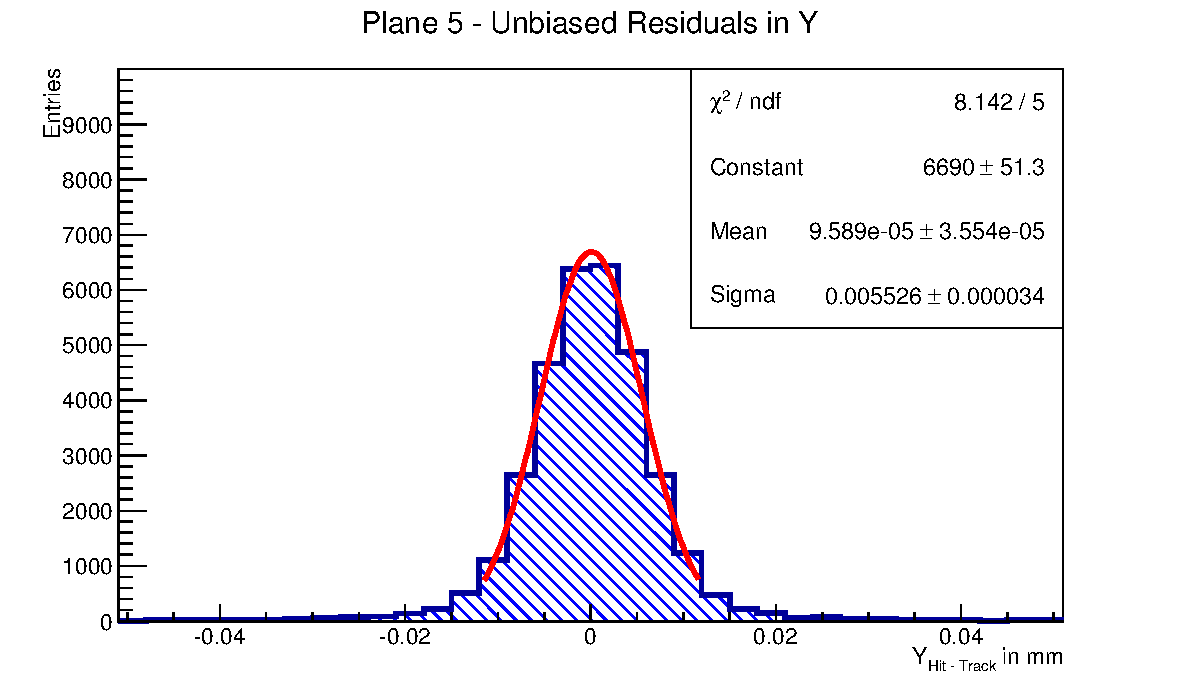
\includegraphics[width=0.45\textwidth]{gfk/chapter03/resis_downstream/5y.pdf}
\caption[Residual examples to determine the DATURA telescope's
resolution. Upstream lever arm]{Residual examples to determine the DATURA
telescope's resolution from the upstream lever arm. From top to bottom: The
measured residuals for planes $0$, $1$, $2$, $3$, $4$ and $5$, left for $X$
direction, right for $Y$ direction. Each sensor plane was considered as a
passive layer during the track reconstruction.}
\label{fig:residualexample1}
\end{figure}

\begin{comment}

\begin{figure}[hbtp]
\centering


\caption[Residual examples to determine the DATURA telescope's
resolution. Downstream lever arm]{Residual examples to determine the DATURA
telescope's resolution from the downstream lever arm. From top to bottom: The
measured residuals for planes $3$, $4$ and $5$, left for $X$ direction, right
for $Y$ direction. Each sensor plane was considered as a passive layer during
the track reconstruction.}
\label{fig:residualexample2}
\end{figure}

\end{comment}

By using a $\chi^{2}$ minimization method, the intrinsic resolution of the
{MIMOSA 26} telescope sensors was calculated from
equation~\ref{eq:telescoperesolutionequation_2}. The results for both a tighter
plane spacing of $20\,\milli\meter$ and a wider spacing of $150\,\milli\meter$
are shown in figures~\ref{fig:smileythin} and~\ref{fig:smileythick},
respectively.\\

\begin{figure}[hbtp]
\centering
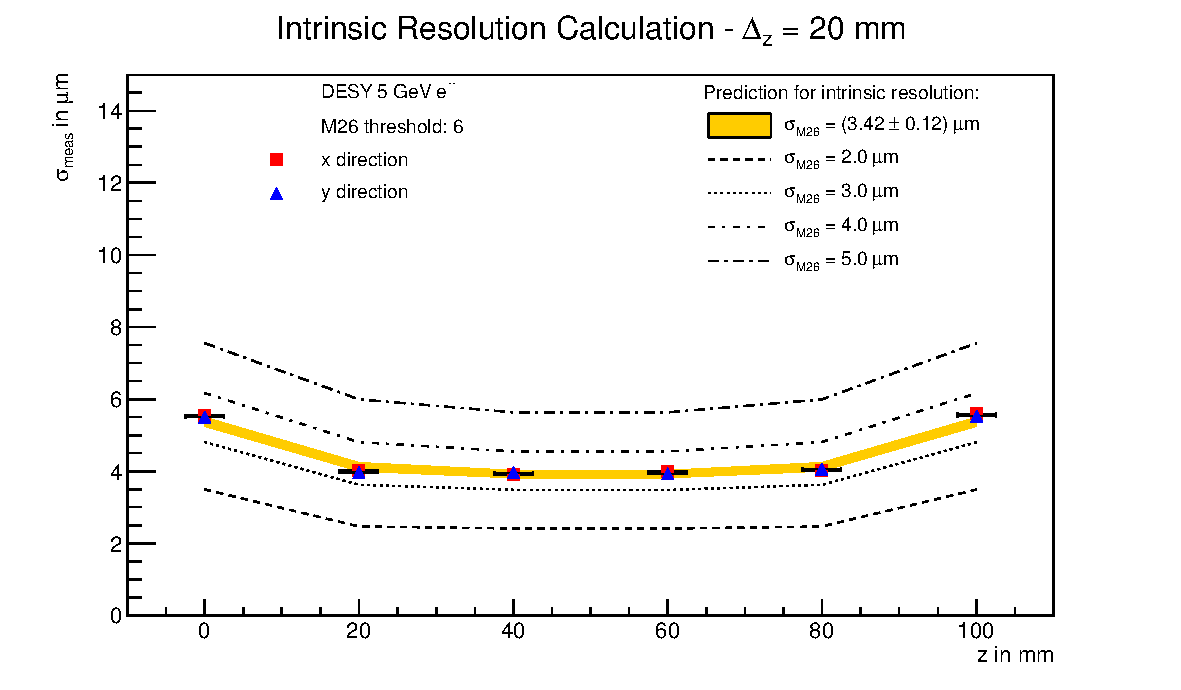
\includegraphics[width=\textwidth]{gfk/chapter03/thin_smiley.pdf}
\caption[Intrinsic telescope sensor resolution at $20\,\milli\meter$ plane
spacing]{Intrinsic telescope sensor resolution at $20\,\milli\meter$ plane
spacing.}
\label{fig:smileythin}
\end{figure}



\begin{figure}[hbtp]
\centering
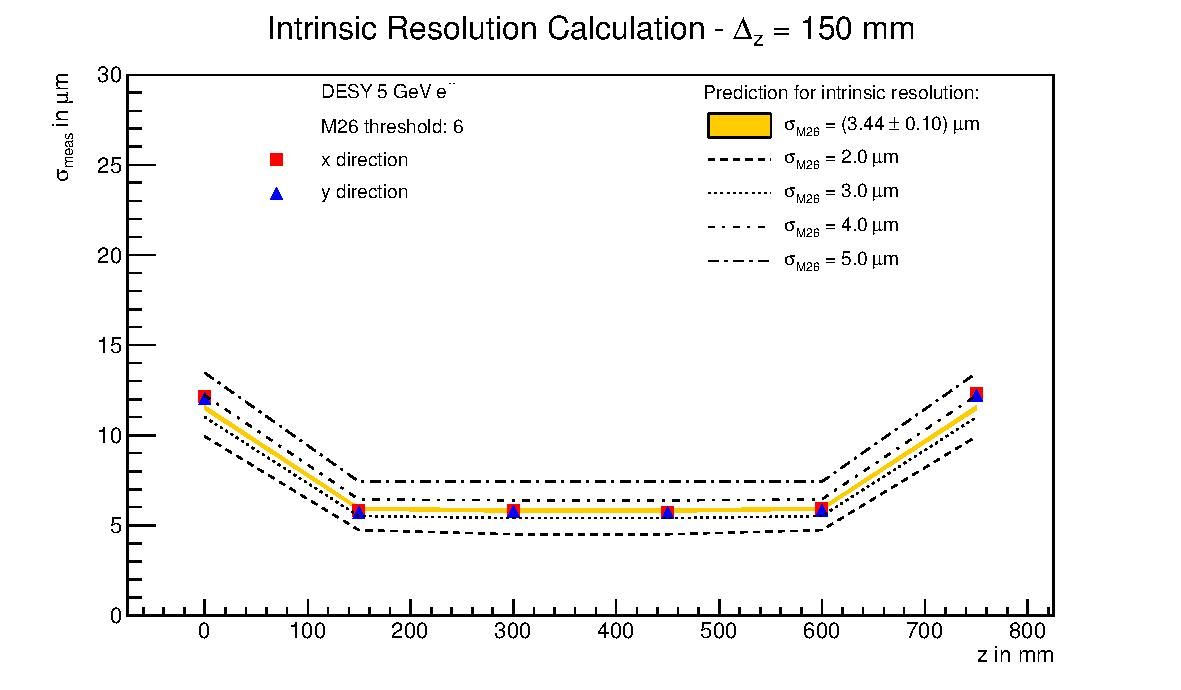
\includegraphics[width=\textwidth]{gfk/chapter03/wide_smiley.pdf}
\caption[Intrinsic telescope sensor resolution at $150\,\milli\meter$ plane
spacing]{Intrinsic telescope sensor resolution at $150\,\milli\meter$ plane
spacing.}
\label{fig:smileythick}
\end{figure}

In both cases, an error of $2.5\,\milli\meter$ on the plane distance
$\Delta_\textrm{z}$ was assumed. The predicted intrinsic resolution
$\sigma_{\textrm{M26}} = \sigma_{\textrm{Intrinsic}}$ of the MIMOSA 26 sensors
is \allowbreak$\left( 3.42\,\pm\, \allowbreak 0.12 \right)\,\micro\meter$ for a
plane spacing of
$20\,\milli\meter$, $\left( 3.44\,\pm\,0.10 \right)\,\micro\meter$ for a plane
spacing of $150\,\milli\meter$. For both geometries, the expected resolution of
$\approx\,3.5\,\micro\meter$, according to~\cite{ref:mimosa26}, can be
confirmed. The underlying assumptions in the method presented here are:\\

\begin{itemize}
\item The intrinsic resolution $\sigma_{\textrm{Intrinsic}}$ of all sensor
planes is assumed to be equal. As the discriminator thresholds are set for
subframes of each plane individually, however, this is not necessarily true.
Figure~\ref{fig:resivsenergy} shows the dependence of
$\sigma_{\textrm{Intrinsic}}$ on the applied threshold.\\

\item The multiple scattering term in
equation~\ref{eq:telescoperesolutionequation_2} is only calculated considering
the nominal sensor thicknesses, the air between sensor planes, and a
$25\,\micro\meter$ thick capton foil on either side of each sensor. The particle
momentum assumed is the nominal beam momentum.\\

\item Residuals are calculated using straight-line tracks only. Inclined tracks,
or a deflection of tracks in planes or scattering material, are not
considered.\\
\end{itemize}

\begin{figure}[hbtp]
\centering

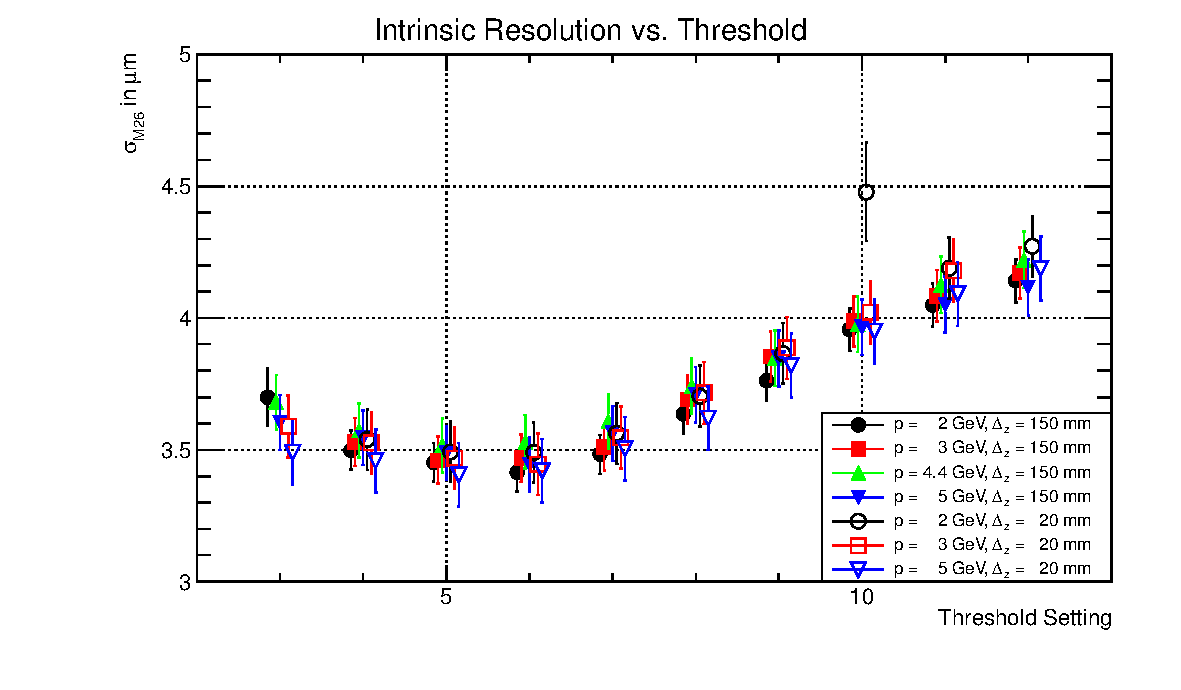
\includegraphics[width=\textwidth]{gfk/chapter03/resi_thresh_errors.pdf}
\caption[Telescope intrinsic sensor resolution for different threshold settings,
beam momenta and geometries]{The measured intrinsic resolution of the DATURA
telescope's MIMOSA 26 sensors $\sigma_{\textrm{M26}}$ for different beam momenta
p, sensor spacing $\Delta_{\textrm{z}}$ and applied sensor threshold. Some
values are shifted on the x-axis for improved legibility.}
\label{fig:resivsenergy}
\end{figure}

Figure~\ref{fig:resivsenergy} shows the calculated intrinsic telescope sensor
resolution for different beam energies, plane distances and applied sensor
thresholds. The minimum of the MIMOSA 26 sensors' intrinsic resolution is
reached for a threshold setting of $6$. While the measured residual width for
wider sensor spacings or lower beam momenta is higher, as can be seen in
figures~\ref{fig:smileythin} and~\ref{fig:smileythick}, these effects are
accounted for in equation~\ref{eq:telescoperesolutionequation} by the terms
$\sigma_{\textrm{Tel}}^2$ and $\sigma_{\textrm{MS}}^2$. Because of this, the
difference in intrinsic sensor resolution between configurations at any given
threshold is only approximately $\pm\,0.15\,\micro\meter$, which is well within
the errors.\\


Measurements by Behr~\cite{ref:j.behrmeasurements}, taken at high thresholds
$>\,10$ show comparable results of $\sigma_{\textrm{M26}} =
(4.35\,\pm\,0.10)\,\micro\meter$. Extrapolating to infinite energies, as
suggested in~\cite{ref:cmosbeamtest} and~\cite{ref:moritzthesis} by a fit over
the inverse square energy, to measure the intrinsic telescope sensor resolution
without multiple scattering effects, was not entirely successfull. This is in
parts due to the uncertainty of the beam energy, caused by deviations in the
dipole magnet current, as shown in~\cite{ref:summerstudentbrm}\\

The signal-to-noise threshold applied to each telescope sensor is a critical
parameter for a telescope's performance. A higher threshold will cut into the
signal, thus reducing the amount of clusters found on each plane and therefore
reducing the amount of reconstructable tracks. This reduces a sensor's
efficiency. A lower threshold will allow an increasing amount of noise hits to
be wrongly identified as clusters. This again will also lead to a broadening of
the residual distributions. Figure~\ref{fig:effi} shows the efficiency
distribution over a sensor plane. The efficiency is defined as the ratio of hits
being measured in the vicinity of a traversing track to the overall number of
tracks. $100\,\micro\meter$ was considered as maximum distance. A noisy pixel
column at $\approx Y = -8\,\milli\meter$ can be observed. This column was masked
during the converter step in the \texttt{datura-noDUT} example and subsequently
is not used during the analysis. Disregarding this area, an overall average
efficiency over $98\,\%$ is observed.\\

\begin{figure}[hbtp]
\centering
\includegraphics[width=\textwidth]{gfk/chapter03/plane3_effi_run37.pdf}
\caption[Telescope sensor efficiency]{Efficiency of telescope sensor plane $3$
at a threshold of $7$ and $5\,\giga\electronvolt$ beam momentum.}
\label{fig:effi}
\end{figure}

In figure~\ref{fig:effi_thresh}, the efficiency dependence on the sensor
threshold is shown, for various beam momenta and sensor spacings. Efficiencies
are averaged for all six sensor planes and both spatial coordinates. In all
cases, the efficiency is $\ge\,98\,\%$ up to a threshold setting of 7. With
increasing threshold, the efficiency declines, until an efficiency of $86\,\%$
for threshold $12$ is reached. The difference between momenta and plane spacings
is due to multiple scattering and increased telescope resolution.\\

\begin{figure}[hbtp]
\centering
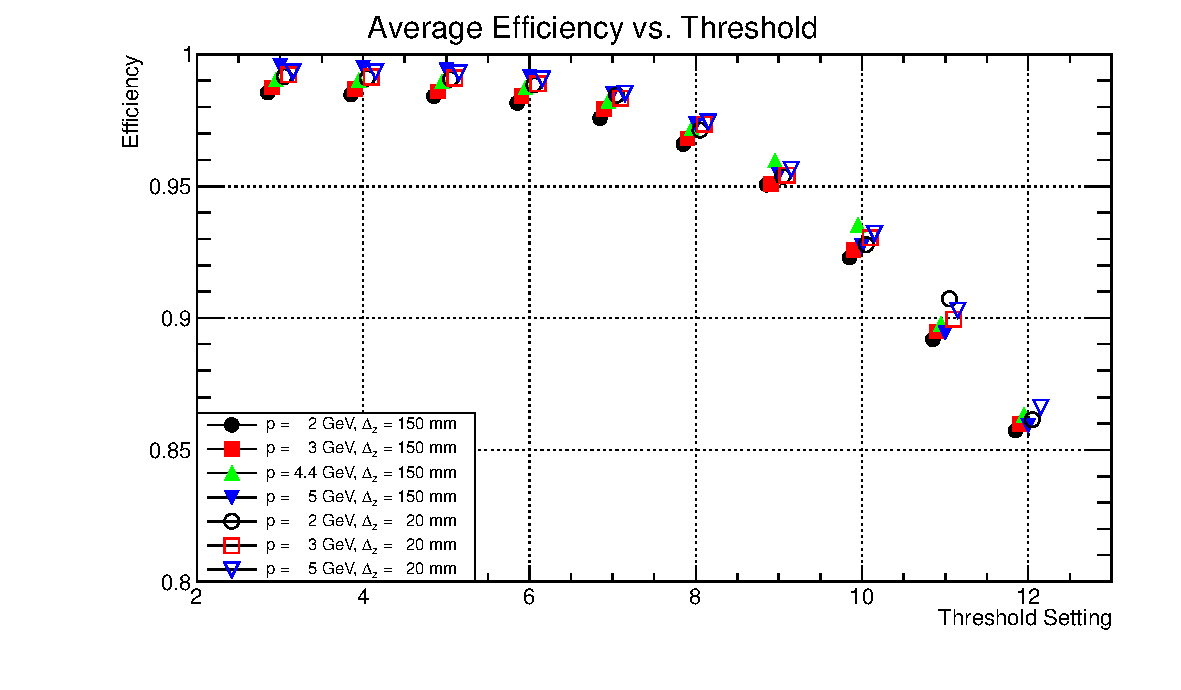
\includegraphics[width=\textwidth]{gfk/chapter03/effi_thresh.pdf}
\caption[Overall telescope sensor efficiency vs. threshold for different beam
momenta and sensor spacings]{Average efficiency of all telescope sensors in both
dimensions for different beam momenta and sensor spacing vs. applied threshold.
An efficiency decline with increasing threshold can be observed. Some values are
shifted on the x-axis for improved legibility.}
\label{fig:effi_thresh}
\end{figure}

